\documentclass[t,usepdftitle=false]{beamer}
\usepackage[utf8]{inputenc}
\usetheme{Warsaw}
\usepackage{xcolor}

\usepackage{etex}
\usepackage{pictex}
\usepackage{tikz}
\usetikzlibrary{shapes,arrows}
\usepackage{pgfplots}

\usepackage{amsmath}
\usepackage{amscd}
\usepackage{pstricks, pst-node}

\usepackage{times}

\usepackage{ulem}

\usepackage{amsmath, amsthm}
\usepackage{listings}

% \setbeamercovered{transparent}
%\usecolortheme{crane}
\title[IFT3245]{IFT 3245\\Simulation et modèles}
\author[Fabian Bastin]{Fabian Bastin\\DIRO\\Université de Montréal}
\date{Automne 2016}

\def\be{\boldsymbol{e}}
\def\bh{\boldsymbol{h}}
\def\bu{\boldsymbol{u}}
\def\bv{\boldsymbol{v}}
\def\bx{\boldsymbol{x}}
\def\by{\boldsymbol{y}}
\def\bA{\boldsymbol{A}}
\def\bB{\boldsymbol{B}}

\def\cJ{\mathcal{J}}
\def\cS{\mathcal{S}}

\def\rit{\mathcal{R}}
\def\RR{\mathcal{R}}
\def\ZZ{\mathcal{Z}}

\begin{document}
\frame{\titlepage}

\begin{frame}
\frametitle{Récurrences linéaires dans $\mathcal{F}_2$}

Considérons $\mathcal{F}_2$, l'ensemble $\lbrace 0, 1 \rbrace$ sur
lequel sont définies les opérations d'addition et de multiplication
modulo 2.

\mbox{}

En d'autres termes, 
\begin{itemize}
\item
l'addition revient à appliquer la porte logique XOR
\item
la multiplication revient à appliquer la porte logique AND
\end{itemize}

\end{frame}

\begin{frame}
\frametitle{Récurrences linéaires dans $\mathcal{F}_2$}

\`A partir du vecteur d'état $\bx_{n-1}$, à l'étape $n-1$, nous
définissons comme précédemment la récurrence linéaire:
\[
 {\bx_n} = {X} \bx_{n-1}.
\]

\mbox{}

Toutefois, $\bx_n$ est exprimé à présent comme un vecteurs de $k$
bits, de sorte que chaque composante se trouve bien dans $\mathcal{F}_2$.
Par exemple, $\bx_n = (0,1,1,0,0,1,0,1,1,0).$

\mbox{}

Le vecteur de sortie $y_n$, défini sur $w$ bits, est obtenu comme suit
\[
 {\by_n} = {B} \bx_{n}.
\]

\end{frame}

\begin{frame}
\frametitle{Récurrences linéaires dans $\mathcal{F}_2$}

Il nous reste à définir la sortie, à savoir un réel compris dans
l'intervalle $[0, 1)$:
\[
 {u_n}  = \sum_{j=1}^w y_{n,j-1} 2^{-j}
       ~=~  .y_{n,0}\; y_{n,1}\; y_{n,2}\; \cdots
\]

\mbox{}

Chaque coordonnée de $\bx_n$ et de $\by_n$ suit la récurrence linéaire
$$
  x_{n,j} = (\alpha_1 x_{n-1,j} + \cdots + \alpha_k x_{n-k,j})\text{ mod }2,
$$
où $\alpha_1, \alpha_2,\ldots, \alpha_k \in \lbrace 0, 1 \rbrace$, ce qui permet de
définir le polynôme caractéristique
$$
  {P(z)} = z^k - \alpha_1 z^{k-1} - \cdots - \alpha_{k-1} z - \alpha_k
             = \det(X-zI).
$$

\mbox{}

La période maximale $\rho = 2^k-1$ est atteinte ssi 
$P(z)$ est primitif sur $\mathcal{F}_2$ (c'est-à-dire qu'il n'est pas
factorisable en produit de polynômes).

\end{frame}

\begin{frame}
\frametitle{Récurrences linéaires dans $\mathcal{F}_2$}

De même que pour les MRG's, il est possible de sauter en avant dans le
séquence ainsi produite, par blocs de ${i}$ étapes, en procédant comme
suit:
\[
 \bx_{n+i} = {\underbrace{(X^i \mod 2)}_{
           \mbox{{\small précalculer}}}} \bx_n \mod 2.
\]

\end{frame}

\begin{frame}
\frametitle{Générateur de Tausworthe (ou LFSR: linear feedback shift register)}

De tels générateurs ont été introduits par Tausworthe, en 1965.
Nous définissons une séquence $x_1, x_2, \ldots$ de chiffres binaires
par la récurrence
\[
 x_n = (a_1 x_{n-1} + \cdots + a_k x_{n-k}) \mod 2,
\]
où $a_1, a_2,\ldots, a_k \in \lbrace 0, 1 \rbrace$, et $a_k \ne 0$.

\mbox{}

Le nom du générateur vient de la possibilité d'utilisation d'un
registre de décalage (shift register), alimenté par une fonction de
feedback linéaire, avec
16 bits. La fonction de sortie est définie comme
\[
 u_n = \sum_{l=1}^w x_{n\nu+l-1} 2^{-l} 
     ~=~ .x_{n\nu} x_{n\nu+1} x_{n\nu+2} \ldots x_{n\nu+w-1}.
\]

\end{frame}

\begin{frame}
\frametitle{Registre de décalage à feedback linéaire.}

\begin{center}
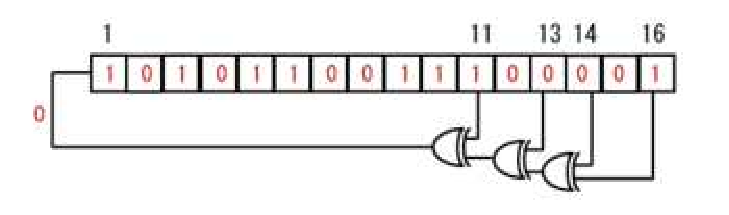
\includegraphics{lfsr_16.pdf}
\end{center}
\label{fig:lfsr}

\end{frame}

\begin{frame}
\frametitle{LFSR}


Cela revient à choisir
\[
 X =
\left(
\begin{tabular}{cccc}
$a_k$    &$a_{k-1}$ & $\ldots$ & $a_1$  \\
1        &          &   & 0     \\
         & $\ddots$ &   & 0      \\
         &          & 1 & 0
\end{tabular}
\right)^\nu \mbox{et } B=I.
\]
Comme précédemment, la période maximale est $\rho = 2^k-1$, laquelle
est atteinte ssi ${Q(z)} = z^k - a_1 z^{k-1} - \cdots - a_{k-1} z - a_k$
est primitif et le plus grand commun diviseur de $\nu$ et $2^k-1$ vaut 1.


\end{frame}

\begin{frame}
\frametitle{LFSR}

Dans la plupart des applications, seulement deux des coefficients sont
non nuls pour simplifier l'implantation, ce qui donne le trinôme:
${Q(z)} = z^k - a_r z^{k-r} - a_k$.

\mbox{}

Comme on travaille dans $\mathcal{F}_2$, cela donne la récurrence
\[
x_n = (x_{n-r}+x_{n-k}) \mod 2.
\]

\mbox{}

L'exécution de l'addition modulo 2 est équivalente à l'instruction
ou-exclusif (xor) sur les bits:
\[
x_n =
\begin{cases}
0 & \mbox{ si } x_{n-r} = x_{n-k},\\
1 & \mbox{ si } x_{n-r} \ne x_{n-k}.
\end{cases}
\]

\end{frame}

\begin{frame}
\frametitle{LFSR}

Plus généralement, on construit une implantation très rapide par des
shifts, xors, masques, etc., si $\nu \le r$ et $2r > k$.

\mbox{}

Les générateurs LFSR sont connus pour avoir des déficiences
statistiques.
On peut cependant en améliorer les propriétés en considérant des LFSR
combinés.

\end{frame}

\begin{frame}
\frametitle{Generalized feedback shift register (GFSR)}

Introduit par Lewis et Payne (1973), ce générateur se base sur la
récurrence
\[
 {\bv_n} = (a_1 \bv_{n-1} + \cdots + a_r \bv_{n-r}) \mod 2 
       ~=~ (v_{n,0},\dots,v_{n,w-1})^T,
\]
et
\[
 \by_n = \bv_{n}.
\]
%   u_n &=& \sum_{j=1}^w v_{n,j-1} 2^{-j}, \mbox{ et}\\

\end{frame}

\begin{frame}
\frametitle{Generalized feedback shift register (GFSR)}

Si $P(z)$ est un trinôme, ce qui est courant dans les implantations, nous avons
\[
 {\bv_n} = (\bv_{n+m-r} + \bv_{n-r}) \mod 2,
\]
ce qui donne
\[
   X =
\left(
\begin{tabular}{cccccc}
   &        &       &  $I_w$ &     & $I_w$ \\
$I_w$&      &       &        &     &    \\
   &  $I_w$ &       &        &     &    \\
   &        & $I_w$ &        &     &    \\
   &        &       &$\ddots$&     &    \\
   &        &       &        &$I_w$&
\end{tabular}
\right)
\]

\end{frame}

\begin{frame}
\frametitle{Generalized feedback shift register (GFSR)}

Plus généralement, ${P(z)} = z^r - a_1 z^{r-1} - \cdots - a_{r-1} z - a_r$
et la période maximale est $2^r-1$ même si l'état a $rw$ bits.

\mbox{}

Ceci signifie que nous utilisons $w$ copies de la récurrence du LFSR, avec des valeurs initiales différentes, et on utilise
une copie pour chaque chiffre de l'expansion fractionnelle de $u_n$.
Si $\lbrace x_{j,n} \rbrace$ désigne la $j^{\mbox{e}}$ copie et si
$x_{j,n} = x_{n+d_j}$ pour tout $j$, $n$,
\[
u_n = \sum_{j = 1}^w x_{n+d_j}2^{-j}.
\]

\mbox{}

Souvent, $d_j = (j-1)d$, pour un certain $d$ fixéé
%, et on revient au cas du trinôme.

\end{frame}

\begin{frame}
\frametitle{Twisted GFSR}

Ces générateurs, proposés par Matsumoto et Kurita 1992, 1994,
généralisent les GFSR comme suit:
\begin {eqnarray*}
 \bv_n &=& (\bv_{n+m-r} + A \bv_{n-r}) \mod 2 \\
 {\by_n} &=& \bv_{n} \mbox{ ou } {\by_n} = {T} \bv_{n}, \\
   X &=&
\left(
\begin{tabular}{cccccc}
   &        &       &  $I_w$ &     & $A$ \\
$I_w$&      &       &        &     &    \\
   &  $I_w$ &       &        &     &    \\
   &        & $I_w$ &        &     &    \\
   &        &       &$\ddots$&     &    \\
   &        &       &        &$I_w$&
\end{tabular}
\right).
\end {eqnarray*}
La période maximale est $2^{rw}-1$, atteinte ssi 
$Q(z^r + z^m)$ est primitif de degré $rw$, où ${Q}$ est le polynôme 
caractéristique de $A$ (i.e. $\det (XI-A)$).
L'exemple le plus connu est le générateur {\tt TT800}, qui atteint une
période de $2^{800}-1$.

\end{frame}

\begin{frame}
\frametitle{Récurrence multiple matricielle}

(Niederreiter 1995)
\begin {eqnarray*}
 \bv_n &=& A_1 \bv_{n-1} + A_2 \bv_{n-2} + \cdots + A_r \bv_{n-r},\\
 {\by_n} &=& \bv_{n}, \\
   X &=&
\left(
\begin{tabular}{ccccc}
$A_1$& $A_2$ & $\ldots$ & $A_{r-1}$ & $A_r$ \\
$I_w$&      &        &     &    \\
   &  $I_w$ &        &     &    \\
   &        &        &     &    \\
   &        &$\ddots$&     &    \\
   &        &        &$I_w$&
\end{tabular}
\right).
\end {eqnarray*}
La période maximale est $2^{rw}-1$.

\end{frame}

\begin{frame}
\frametitle{Mersenne Twister}

La période peut être considérablement améliorée en considérant une
récurrence de la forme
\begin{align*}
 \bv_n &= (\bv_{n+m-r} + A (\bv_{n-r}^{u} | \bv_{n-r+1}^l) \mod
 2, \\
 \by_n &= T \bv_{n}.
\end{align*}

\mbox{}

L'exposant $u$ signifie que nous prenons les $(w-p)$ bits de poids
forts, et $l$, les $p$ bits de poids faible.
Cette relation est connue sous le nom Mersenne Twister, comme
introduit par Matsumoto et Nishimura (1998).

\mbox{}

La récurrence peut être réécrite
\[
 \bv_n = \left( \bv_{n+m-r} + A
 \begin{pmatrix} 0 & 0 \\ 0 & I_p \end{pmatrix} v_{n-r+1}
 \begin{pmatrix} I_{w-p} & 0 \\ 0 & 0 \end{pmatrix} v_{n-r}
  \right) \mod 2,
\]

\end{frame}

\begin{frame}
\frametitle{Mersenne Twister}

Nous pouvons exprimer $X$ comme la matrice $(nw-p)\times(nw-p)$
\begin{eqnarray*}
\left(
\begin{tabular}{ccccccc}
   &        &       &  $I_w$ &     & 0 \\ $A\;\mbox{rot}_p(I)$ \\
$I_w$&      &       &        &     &    \\
   &  $I_w$ &       &        &     &    \\
   &        & $I_w$ &        &     &    \\
   &        &       &$\ddots$&     &    \\
   &        &       &        &$I_w$& 0  & 0\\
 0 &        &       &        &  0  & $I_{w-p}$ & 0 \\
\end{tabular}
\right).
\end {eqnarray*}
en considérant dans le vecteur d'état les $r$ vecteurs
$v_n$,\ldots,$v_{n-r+2}$ ainsi que, de manière répétée, les $p$ bits de
poids fort de $v_{n-r+1}$.

\end{frame}

\begin{frame}
\frametitle{Mersenne Twister}

$\mbox{rot}_p(I)$ est défini comme
\[
\begin{pmatrix}
0 & I_{w-p} \\ I_p & 0
\end{pmatrix}.
\]
La période maximale est $2^{rw-p}-1$.
Un exemple populaire est le générateur {\tt MT19937}, dont la période
de $2^{19937}-1$.

\end{frame}

\begin{frame}
\frametitle{Générateurs combinés sur $\mathcal{F}_2$}

${J}$ générateurs $\mathcal{F}_2$-linéaires de paramétres 
$(k_j, w, \bA_j, \bB_j)$ et états $\bx_{j,i}$.

\mbox{}

\begin{eqnarray*}
 \by_n &=& \bB_1\bx_{1,n} \oplus \cdots \oplus\bB_J\bx_{J,n},
                                                   \label{eq:comba}\\
 u_n   &=& \sum_{\ell=1}^w y_{n,\ell-1} 2^{-\ell}, \label{eq:combb}
\end{eqnarray*}

\mbox{}

Equivalent à un générateur $\mathcal{F}_2$-linéaire 
ayant $k=k_1 + \cdots + k_J$, $\bA =$ diag$(\bA_1,\dots,\bA_J)$, 
et $\bB = (\bB_1,\dots, \bB_J)$.

\end{frame}

\begin{frame}
\frametitle{Générateurs combinés sur $\mathcal{F}_2$}

Si on combine des LFSRs ayant des polynômes caractéristiques $P_j(z)$,
le générateur combiné a comme polynôme caractéristique 
$P(z) = P_1(z)\cdots P_J(z)$ et sa période peut atteindre le produit
des périodes.

\mbox{}

En combinant des LFSR, TGFSR, ou Mersenne twister entre eux, on obtient 
des générateurs ayant de bien meilleures équidistributions.

\end{frame}

\begin{frame}[fragile]
\frametitle{LFSR113}

\begin{lstlisting}
unsigned long z1, z2, z3, z4;

double lfsr113 ()
   {  /* Generates numbers between 0 and 1. */
   unsigned long b;
   b  = (((z1 <<  6) ^ z1) >> 13);
   z1 = (((z1 & 4294967294) << 18) ^ b);
   b  = (((z2 <<  2) ^ z2) >> 27);
   z2 = (((z2 & 4294967288) <<  2) ^ b);
   b  = (((z3 << 13) ^ z3) >> 21);
   z3 = (((z3 & 4294967280) <<  7) ^ b);
   b  = (((z4 <<  3) ^ z4) >> 12);
   z4 = (((z4 & 4294967168) << 13) ^ b);
   return ((z1^z2^z3^z4)*2.3283064365387e-10);
   }
\end{lstlisting} 

\end{frame}

\begin{frame}[fragile]
\frametitle{LFSR113}

Les opérations utilisées sont
\begin{itemize}
\item
$\&$: opérateur et.
\item
$\hat{\ }$: ou exlusif.
\item
$<<$: decale à gauche; revient à multiplier par une puissance de 2.
\item
$>>$: decale à droite; revient à diviser par une puissance de 2. 
\end{itemize}

\end{frame}

\end{document}
